%Folgende Zeile aktivieren und als SVN property "svn:keywords" auf "Id" setzen, um SVN Versionsinformationen im Dokument zu erhalten
%\svnInfo $Id: einleitung.tex 60 2012-01-26 15:56:06Z koppor $ 

\chapter{Selektion gut detektierbarer Bilder}
\label{chap:slk}
	Um aus dem beschriebenen Bilderstack möglichst gut detektierbare Einzelbilder zu erhalten, werden hier verschiedene Verfahren vorgestellt, die weitestgehend automatisch eine Auswahl von Bildern erstellt, die für die weitere Objekterkennung gut geeignet sind. \\
Da der gescannte Mikrochip aus vier Leiterbahnschichten besteht, muss der beim Scannen entstehende Bilderstack in vier Intervalle eingeteilt werden, welches jeweils eine Leiterbahnschicht repräsentiert. 
\begin{figure}[H]
  \begin{center}
    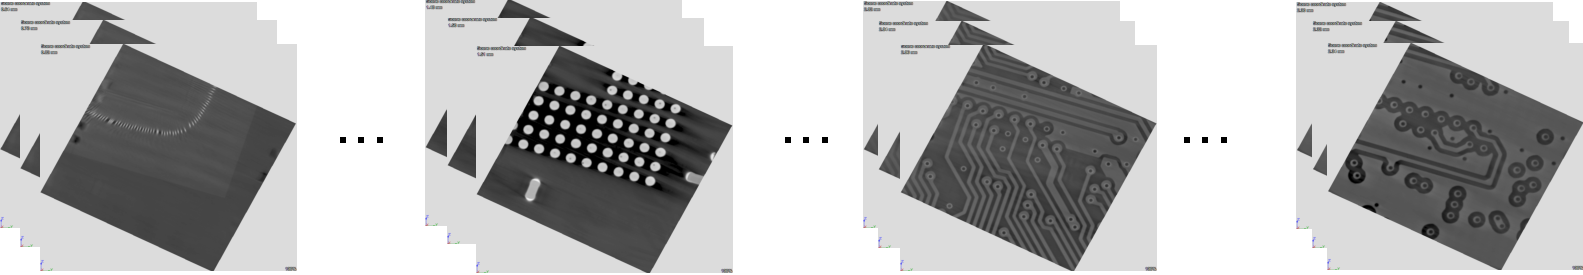
\includegraphics[width=\textwidth]{stack.pdf}
    \caption{Einteilung des Bilderstacks in vier Intervalle}
    \label{fig:intervalls}
  \end{center}
\end{figure}
Ziel der unten vorgestellten Verfahren besteht darin, um für jedes Intervall das Bild zu finden, dass die Leiterbahnschicht am genausten repräsentiert.
Die aus den Verfahren gewonnen Bilder werden anschließend weiterverwendet, d.h. es werden die 2D Objekterkennungsverfahren darauf angewandt und bewertet, wie gut die ausgewählten Bilder für die einzelnen Verfahren geeignet sind, und ob für jedes Intervall tatsächlich das am besten detektierbare Bild gefunden wurde.\\ \\

Um die aufgeführten Verfahren miteinander vergleichen zu können, wird für jedes Intervall das "`Best Match"' vor dem Vergleich ausgewählt. Dabei handelt es sich um jenes Bild, in dem die Objekte am besten sichtbar sind. Für die vier Intervalle sind dies folgende Bilder:

\begin{figure}[H]
  \begin{center}
    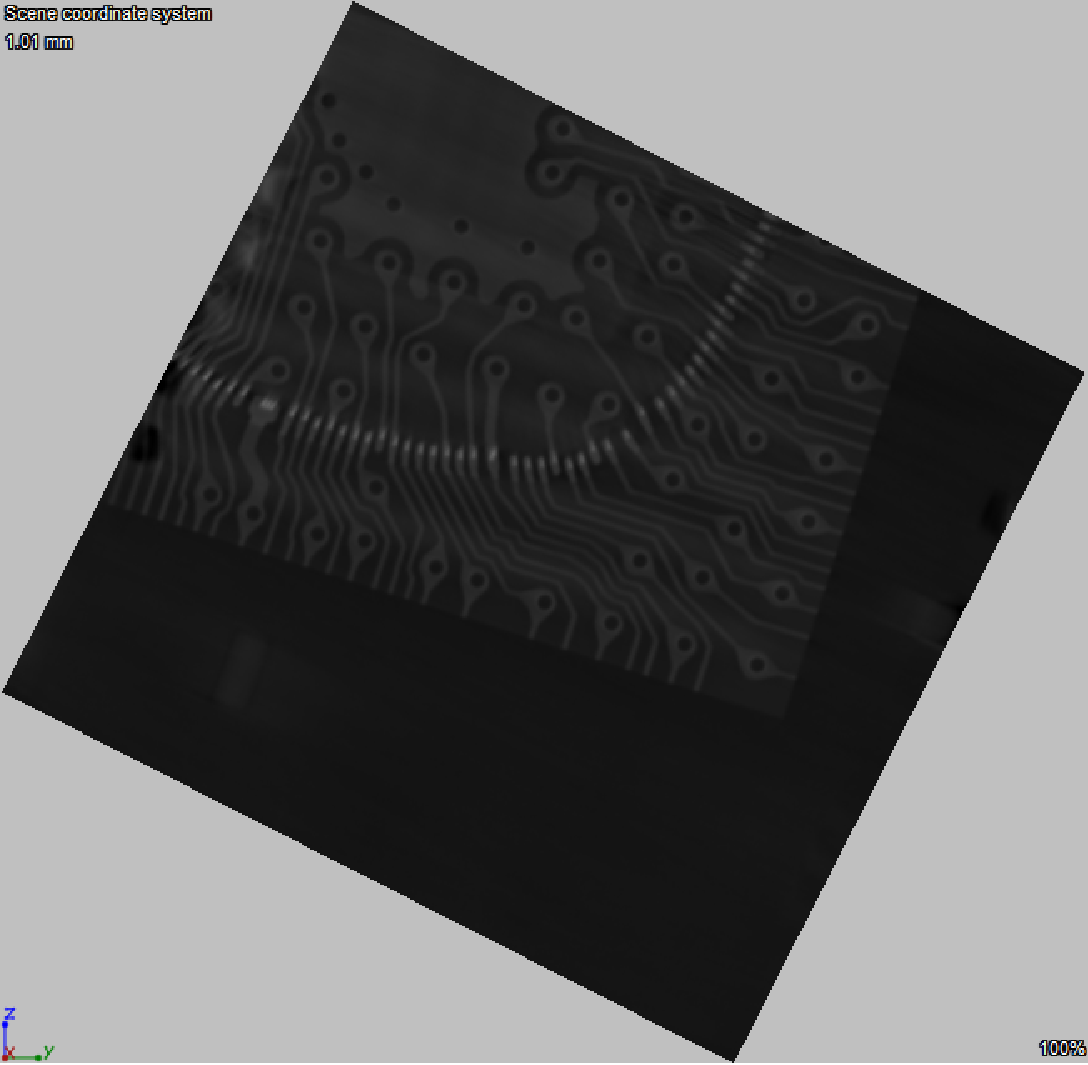
\includegraphics[width=0.5\textwidth]{best1.pdf}
    \caption{Best Match des ersten Intervalls}
    \label{fig:bestmatch1}
  \end{center}
\end{figure}

\begin{figure}[H]
  \begin{center}
    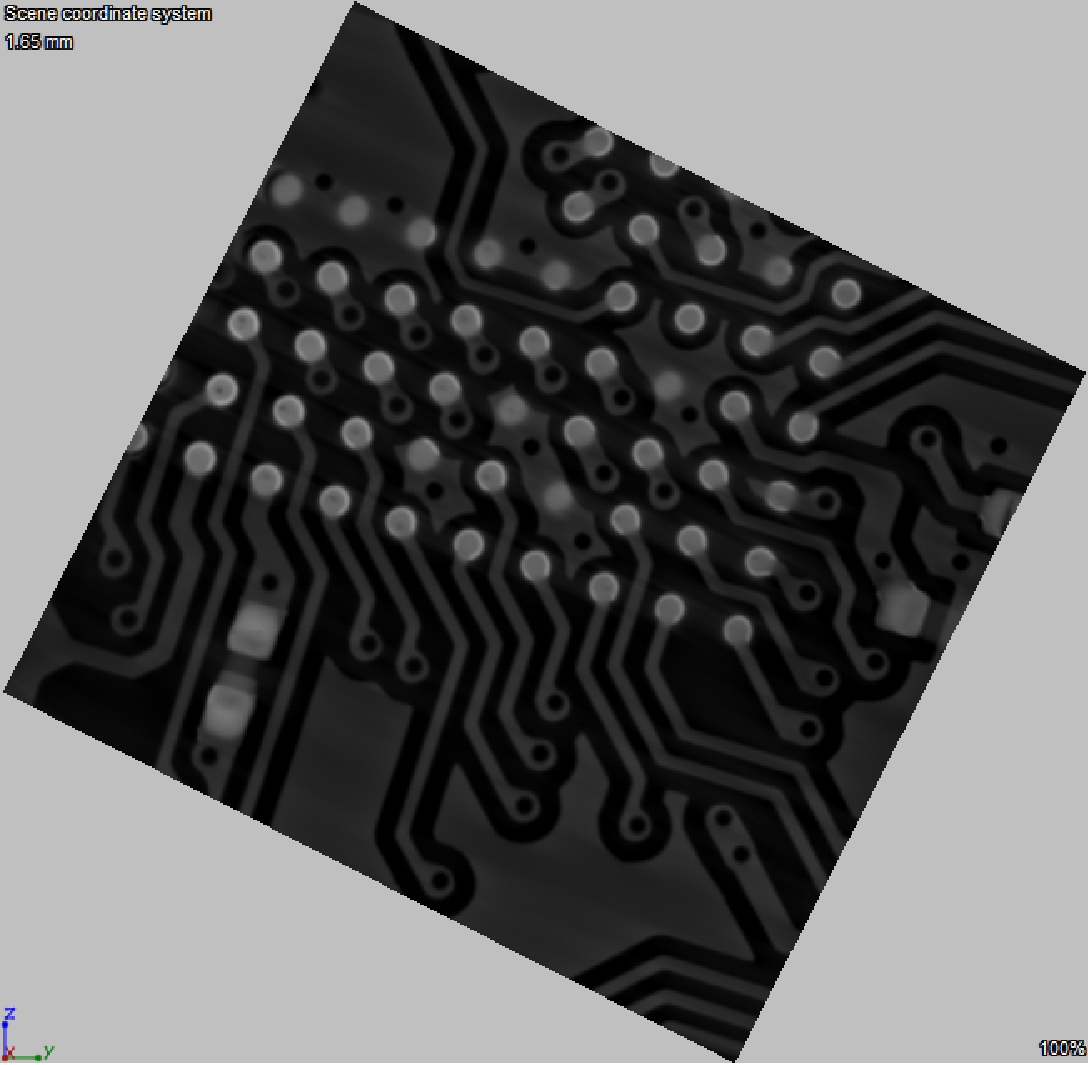
\includegraphics[width=0.5\textwidth]{best2.pdf}
    \caption{Best Match des zweiten Intervalls}
    \label{fig:bestmatch2}
  \end{center}
\end{figure}

\begin{figure}[H]
  \begin{center}
    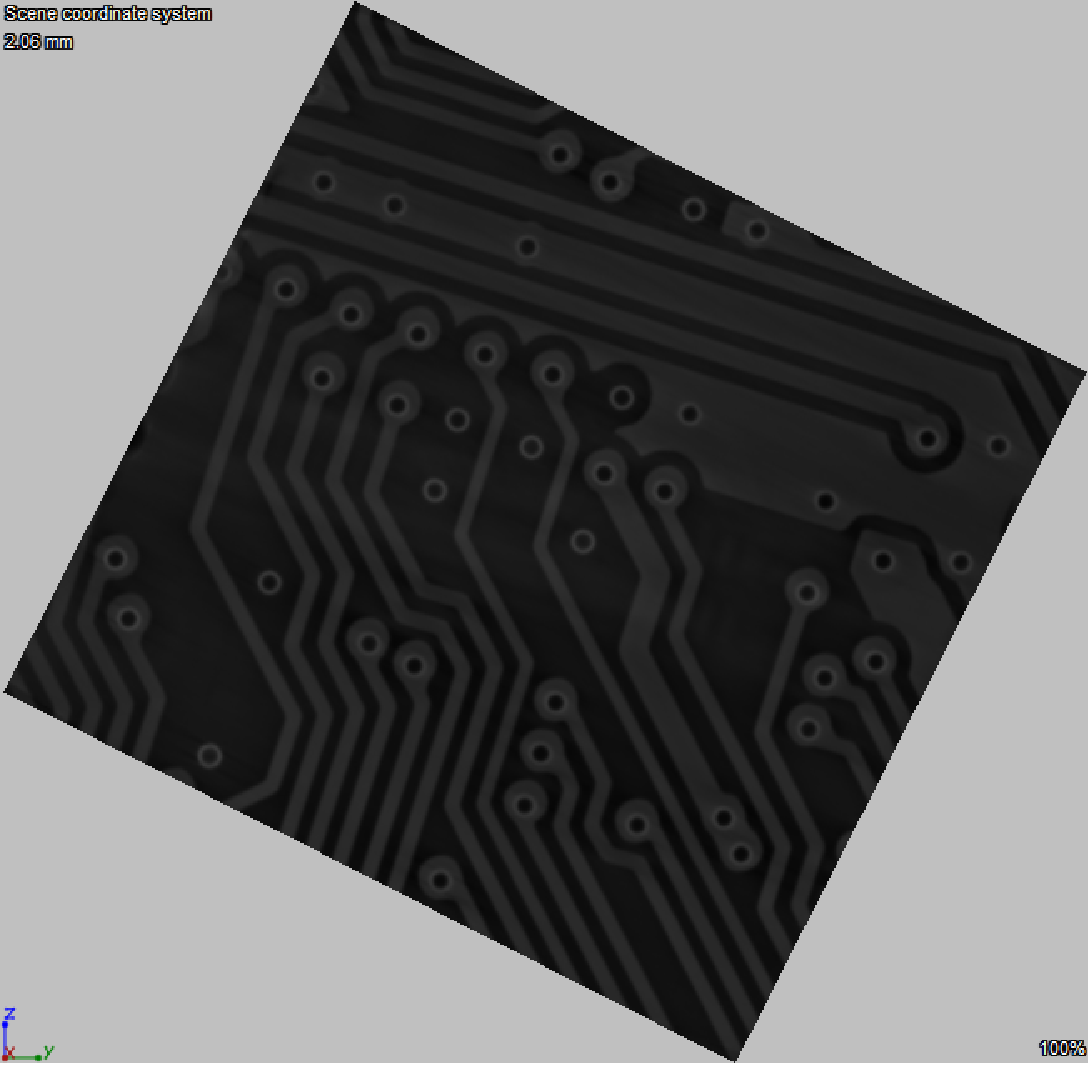
\includegraphics[width=0.5\textwidth]{best3.pdf}
    \caption{Best Match des dritten Intervalls}
    \label{fig:bestmatch3}
  \end{center}
\end{figure}

\begin{figure}[H]
  \begin{center}
    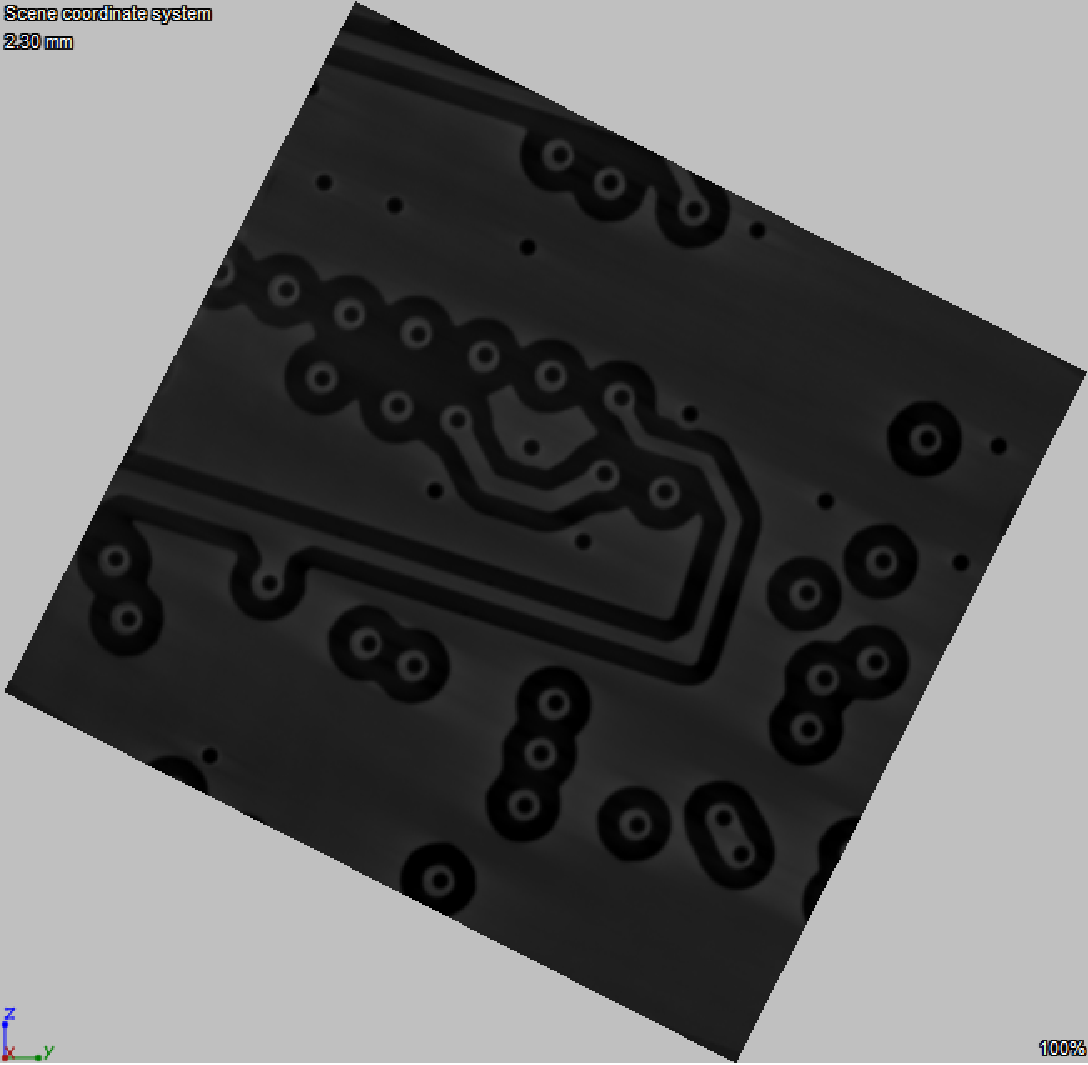
\includegraphics[width=0.5\textwidth]{best4.pdf}
    \caption{Best Match des vierten Intervalls}
    \label{fig:bestmatch4}
  \end{center}
\end{figure}

Diese Best Matches haben im Bilderstack jeweils die Indizes
\begin{enumerate}
	\item{Intervall 1: $Index 27$}
	\item{Intervall 2: $Index 61$}
	\item{Intervall 3: $Index 83$}
	\item{Intervall 4: $Index 96$}
\end{enumerate}

Die Ergebnisse der einzelnen Verfahren werden mit diesen Best Matches verglichen, indem die durschnittliche Distanz der Ergebnisse zu den Best Matches im Bilderstack ermittelt wird. 

\section{Binärbilder}
Bei diesem Verfahren werden zunächst alle Bilder in Binärbilder umgewandelt. Als binärer Schwellwert wird dabei der Wert 70 gewählt, d.h. alle Pixel, deren Grauwert größer als 70 ist, wird der Grauwert 255 zugewiesen, allen Pixeln die einen Grauwert kleiner, bzw. gleich 70 besitzen, wird der Grauwert 0 zugewiesen. Anschließend wird das Bild ausgewählt, welches die maximale Anzahl an weißen Pixeln (Pixel mit dem Grauwert 255) besitzen.

Die Idee, die hinter diesem Verfahren steckt, ist, dass Bilder, die eine möglichst große Anzahl von Pixeln mit maximalen Grauwert besitzen, viele Objekte enthalten, die detektiert werden können. \\
\newpage
\subsection{Ergebnis} 

Die Ergebnisse des Verfahrens für die vier Intervalle:
\begin{figure}[H]
  \begin{center}
    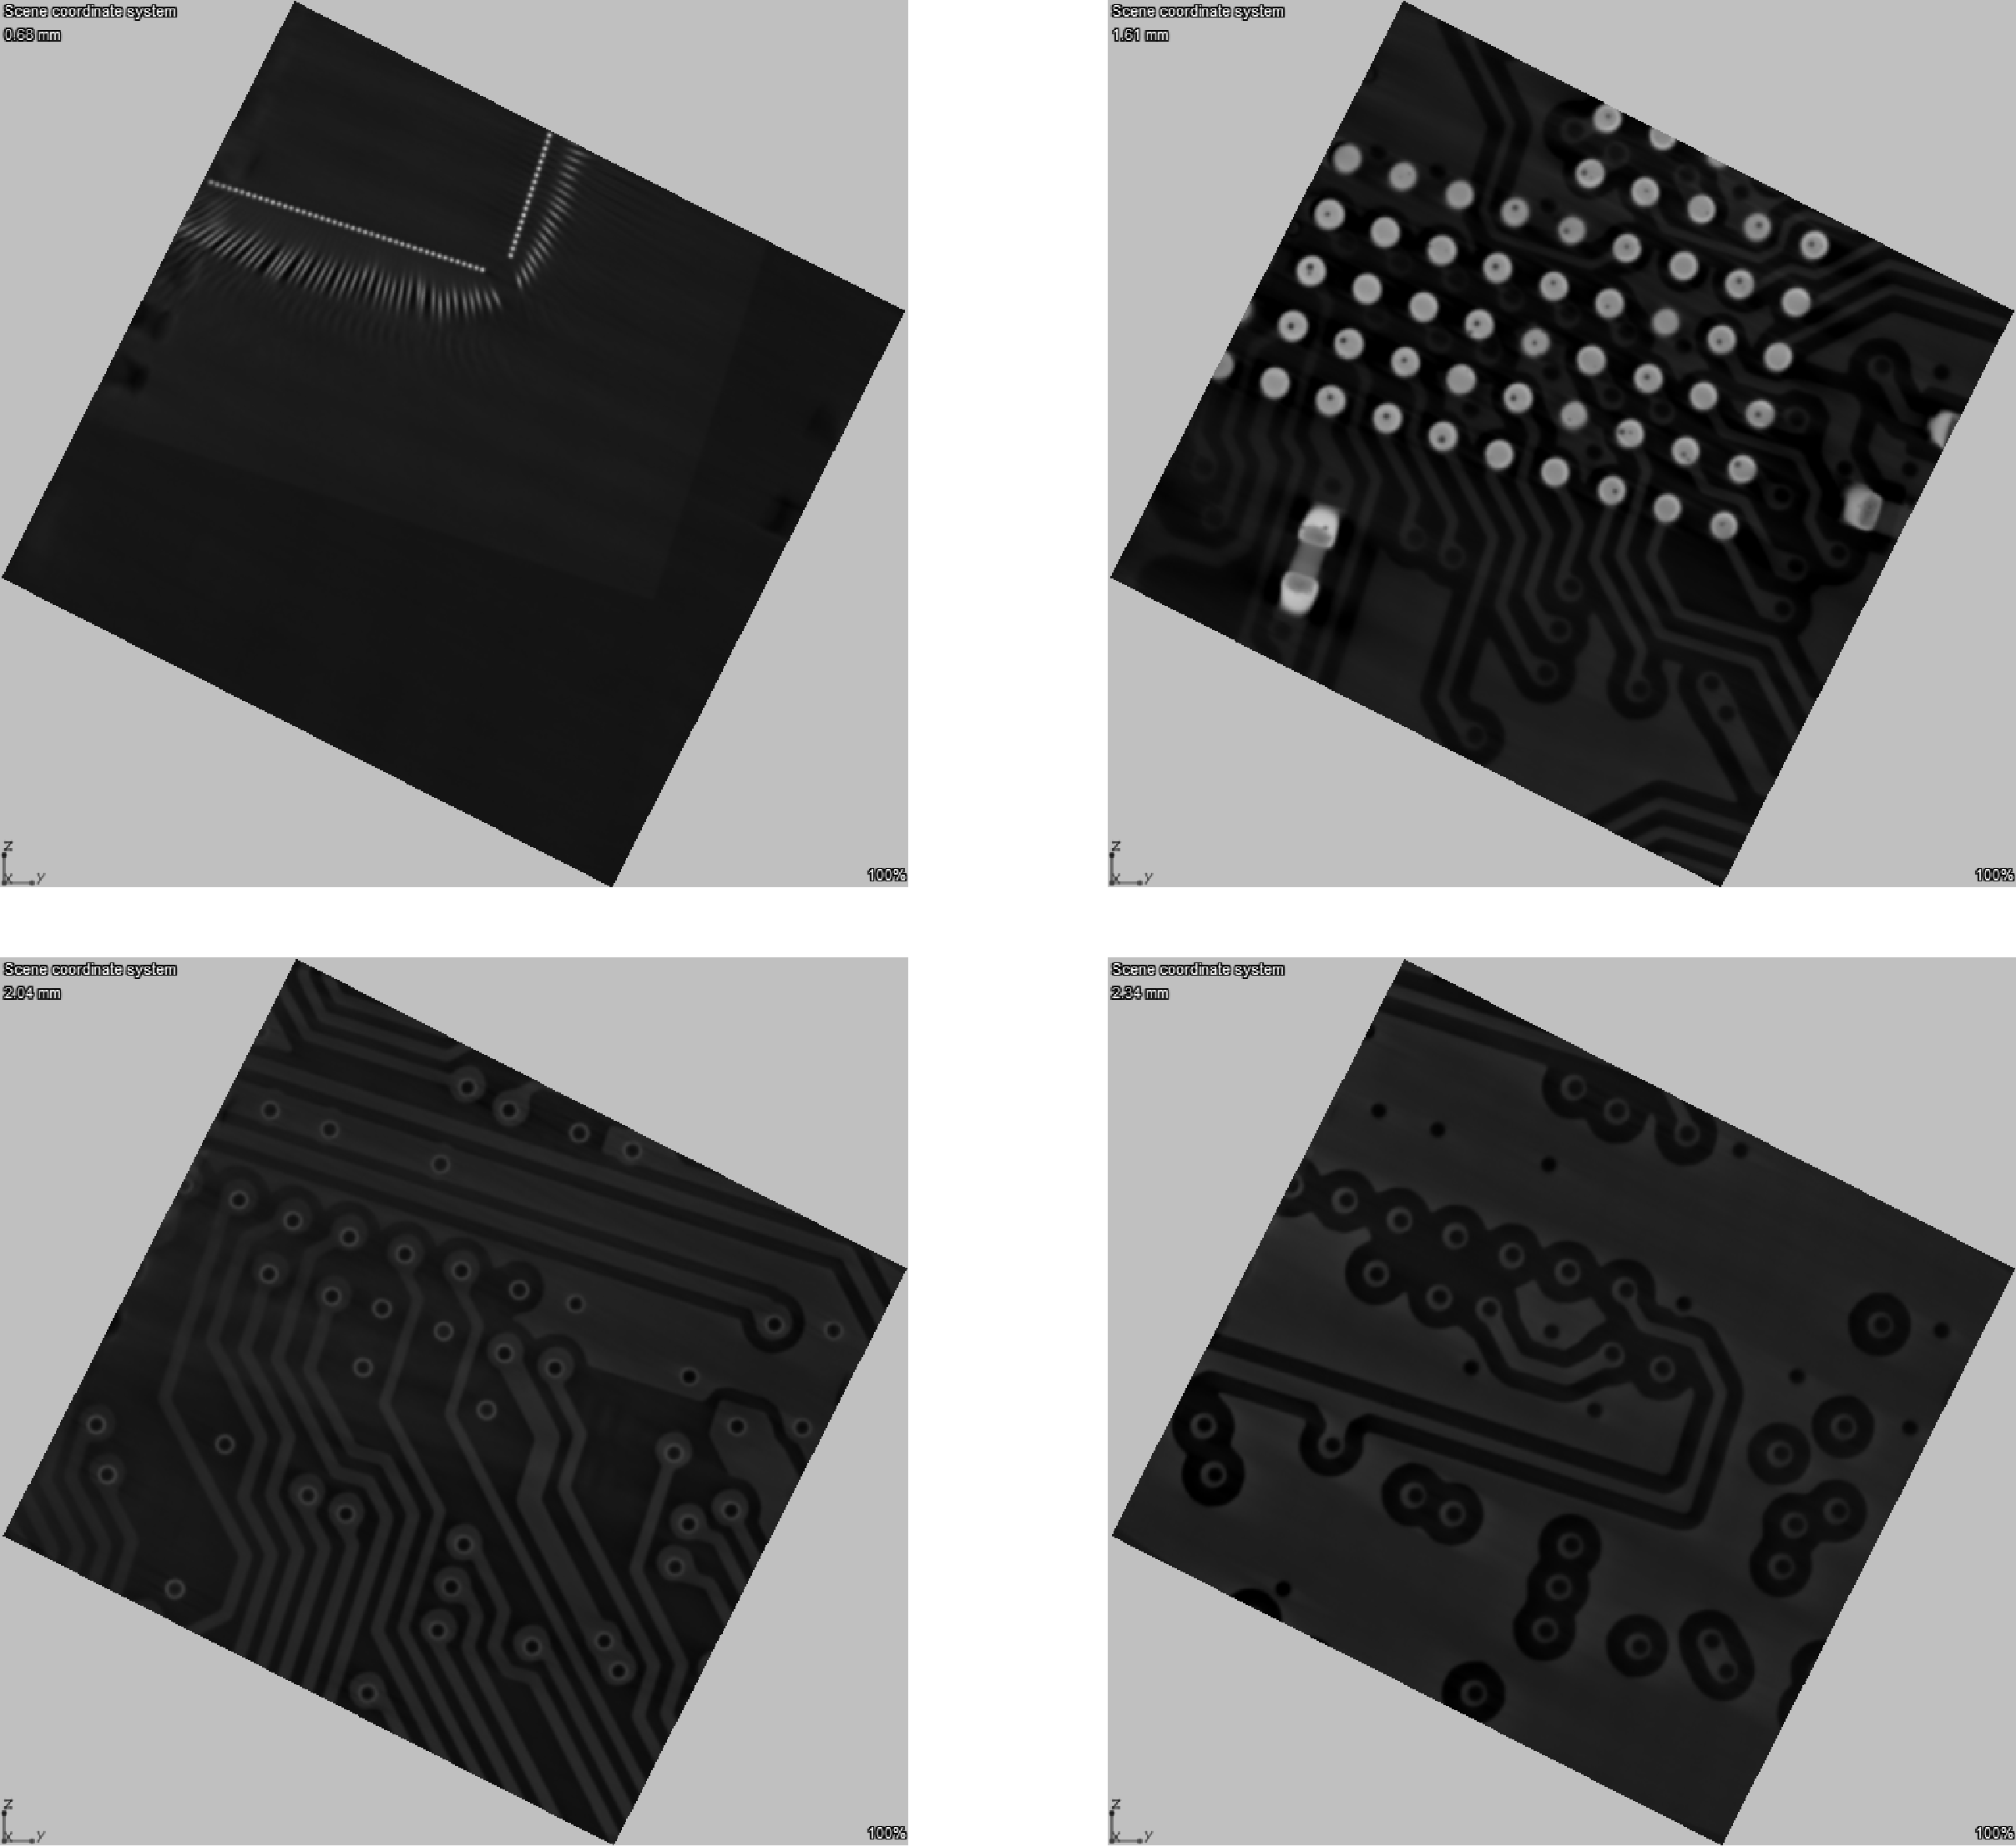
\includegraphics[width=0.9\textwidth]{binary_max.pdf}
    \caption{Ergebnisse des Binärbildverfahrens}
    \label{fig:binary_bestmatch4}
  \end{center}
\end{figure}

Für die einzelnen Intervalle  sind dies die Bilder mit folgenden Indizes:
\begin{enumerate}
	\item{Interval l1: $Index$ $9$ , Differenz zum Best Match: 18}
	\item{Intervall 2: $Index$ $59$, Differenz zum Best Match: 2}
	\item{Intervall 3: $Index$ $82$, Differenz zum Best Match: 1 }
	\item{Intervall 4: $Index$ $98$, Differenz zum Best Match: 2}
\end{enumerate}

Dies führt zu einer durchschnittlichen Distanz von \textbf{5,75} vom Best Match.


\section{Canny-Edge-Bilder}
Bei diesem Verfahren werden die einzelnen Bilder der Intervalle zunächst mit dem Canny-Edge Operator in die entsprechenden Kantenbilder überführt. Anschließend werden die Kantenpixeln in den Kantenbildern gezählt, wobei für jedes Intervall das Bild ausgewählt wird, dass die meisten Kantenpixel besitzt.\\

Der Ansatz hierbei ist, dass Bilder, die viele einzelne Objekte enthalten, mehr Kantenpixel liefern, als Bilder, in denen wenige Objekte enthalten sind.
\newpage
\subsection{Ergebnis} 

Die Ergebnisse des Verfahrens für die vier Intervalle:
\begin{figure}[H]
  \begin{center}
    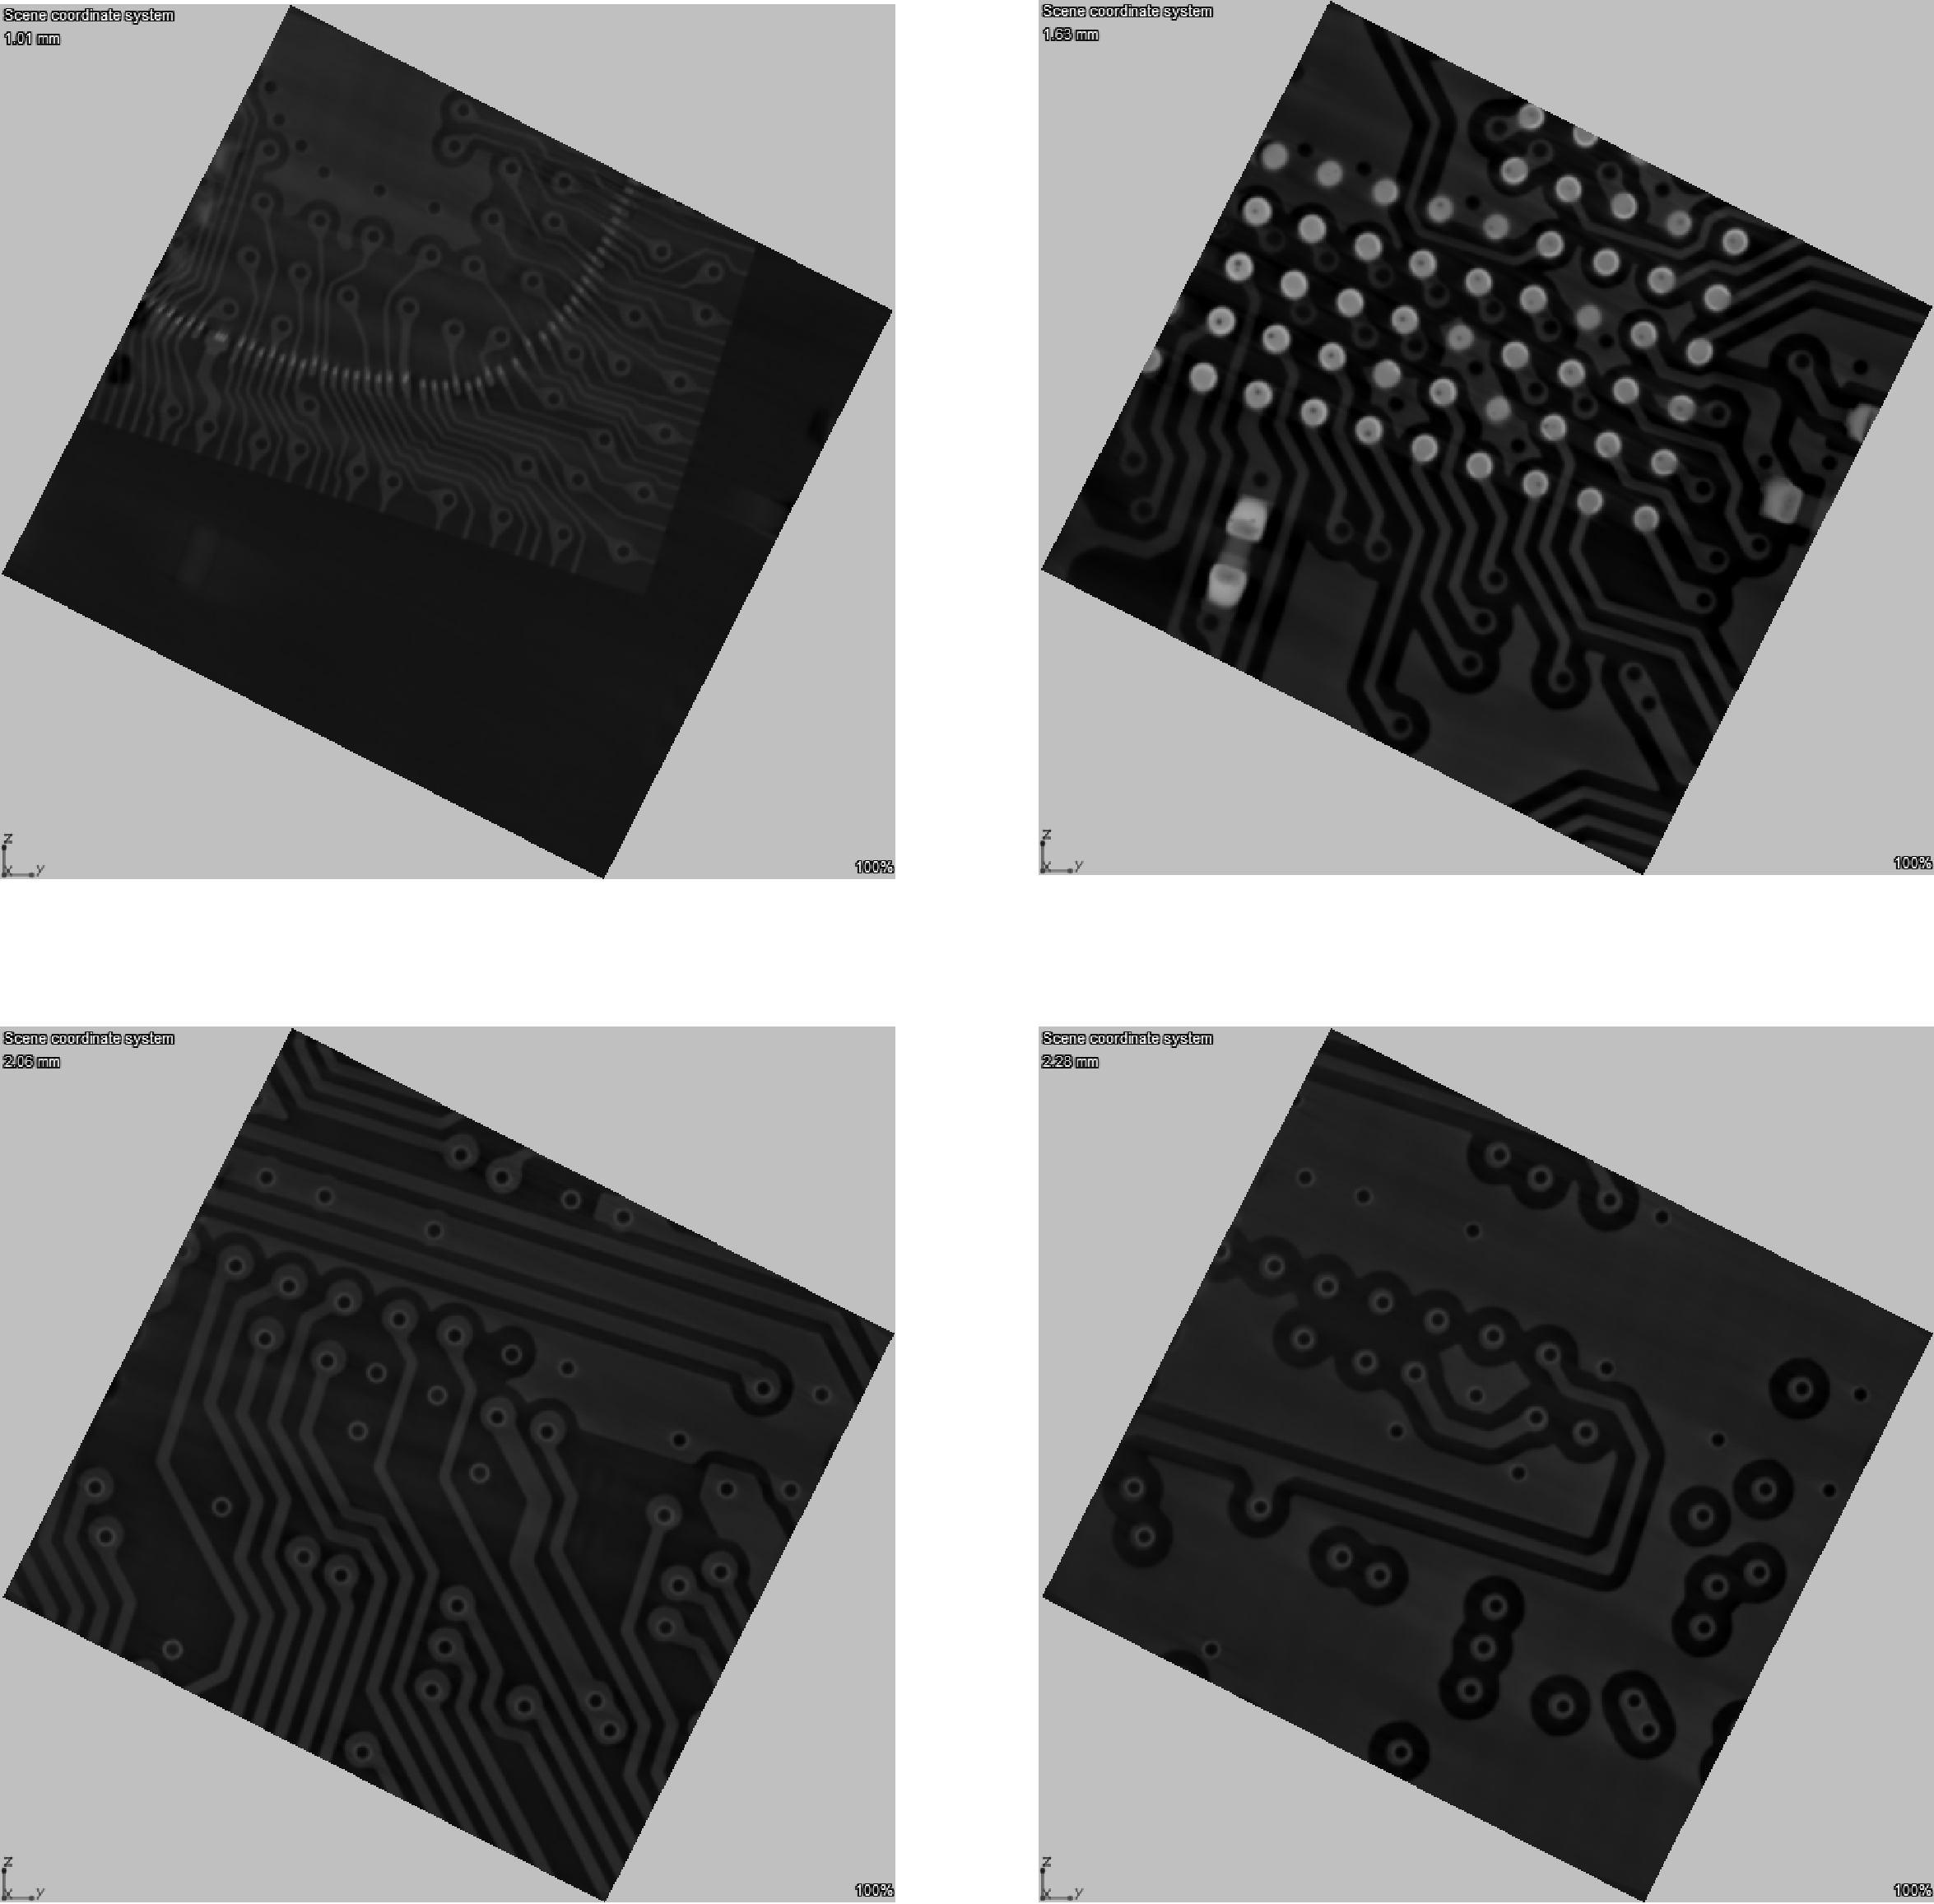
\includegraphics[width=0.9\textwidth]{canny_max_results.pdf}
    \caption{Ergebnisse des Canny-Edge-Verfahrens}
    \label{fig:canny_bestmatch4}
  \end{center}
\end{figure}
\newpage
Die zugehörigen Katenbilder:
\begin{figure}[H]
  \begin{center}
    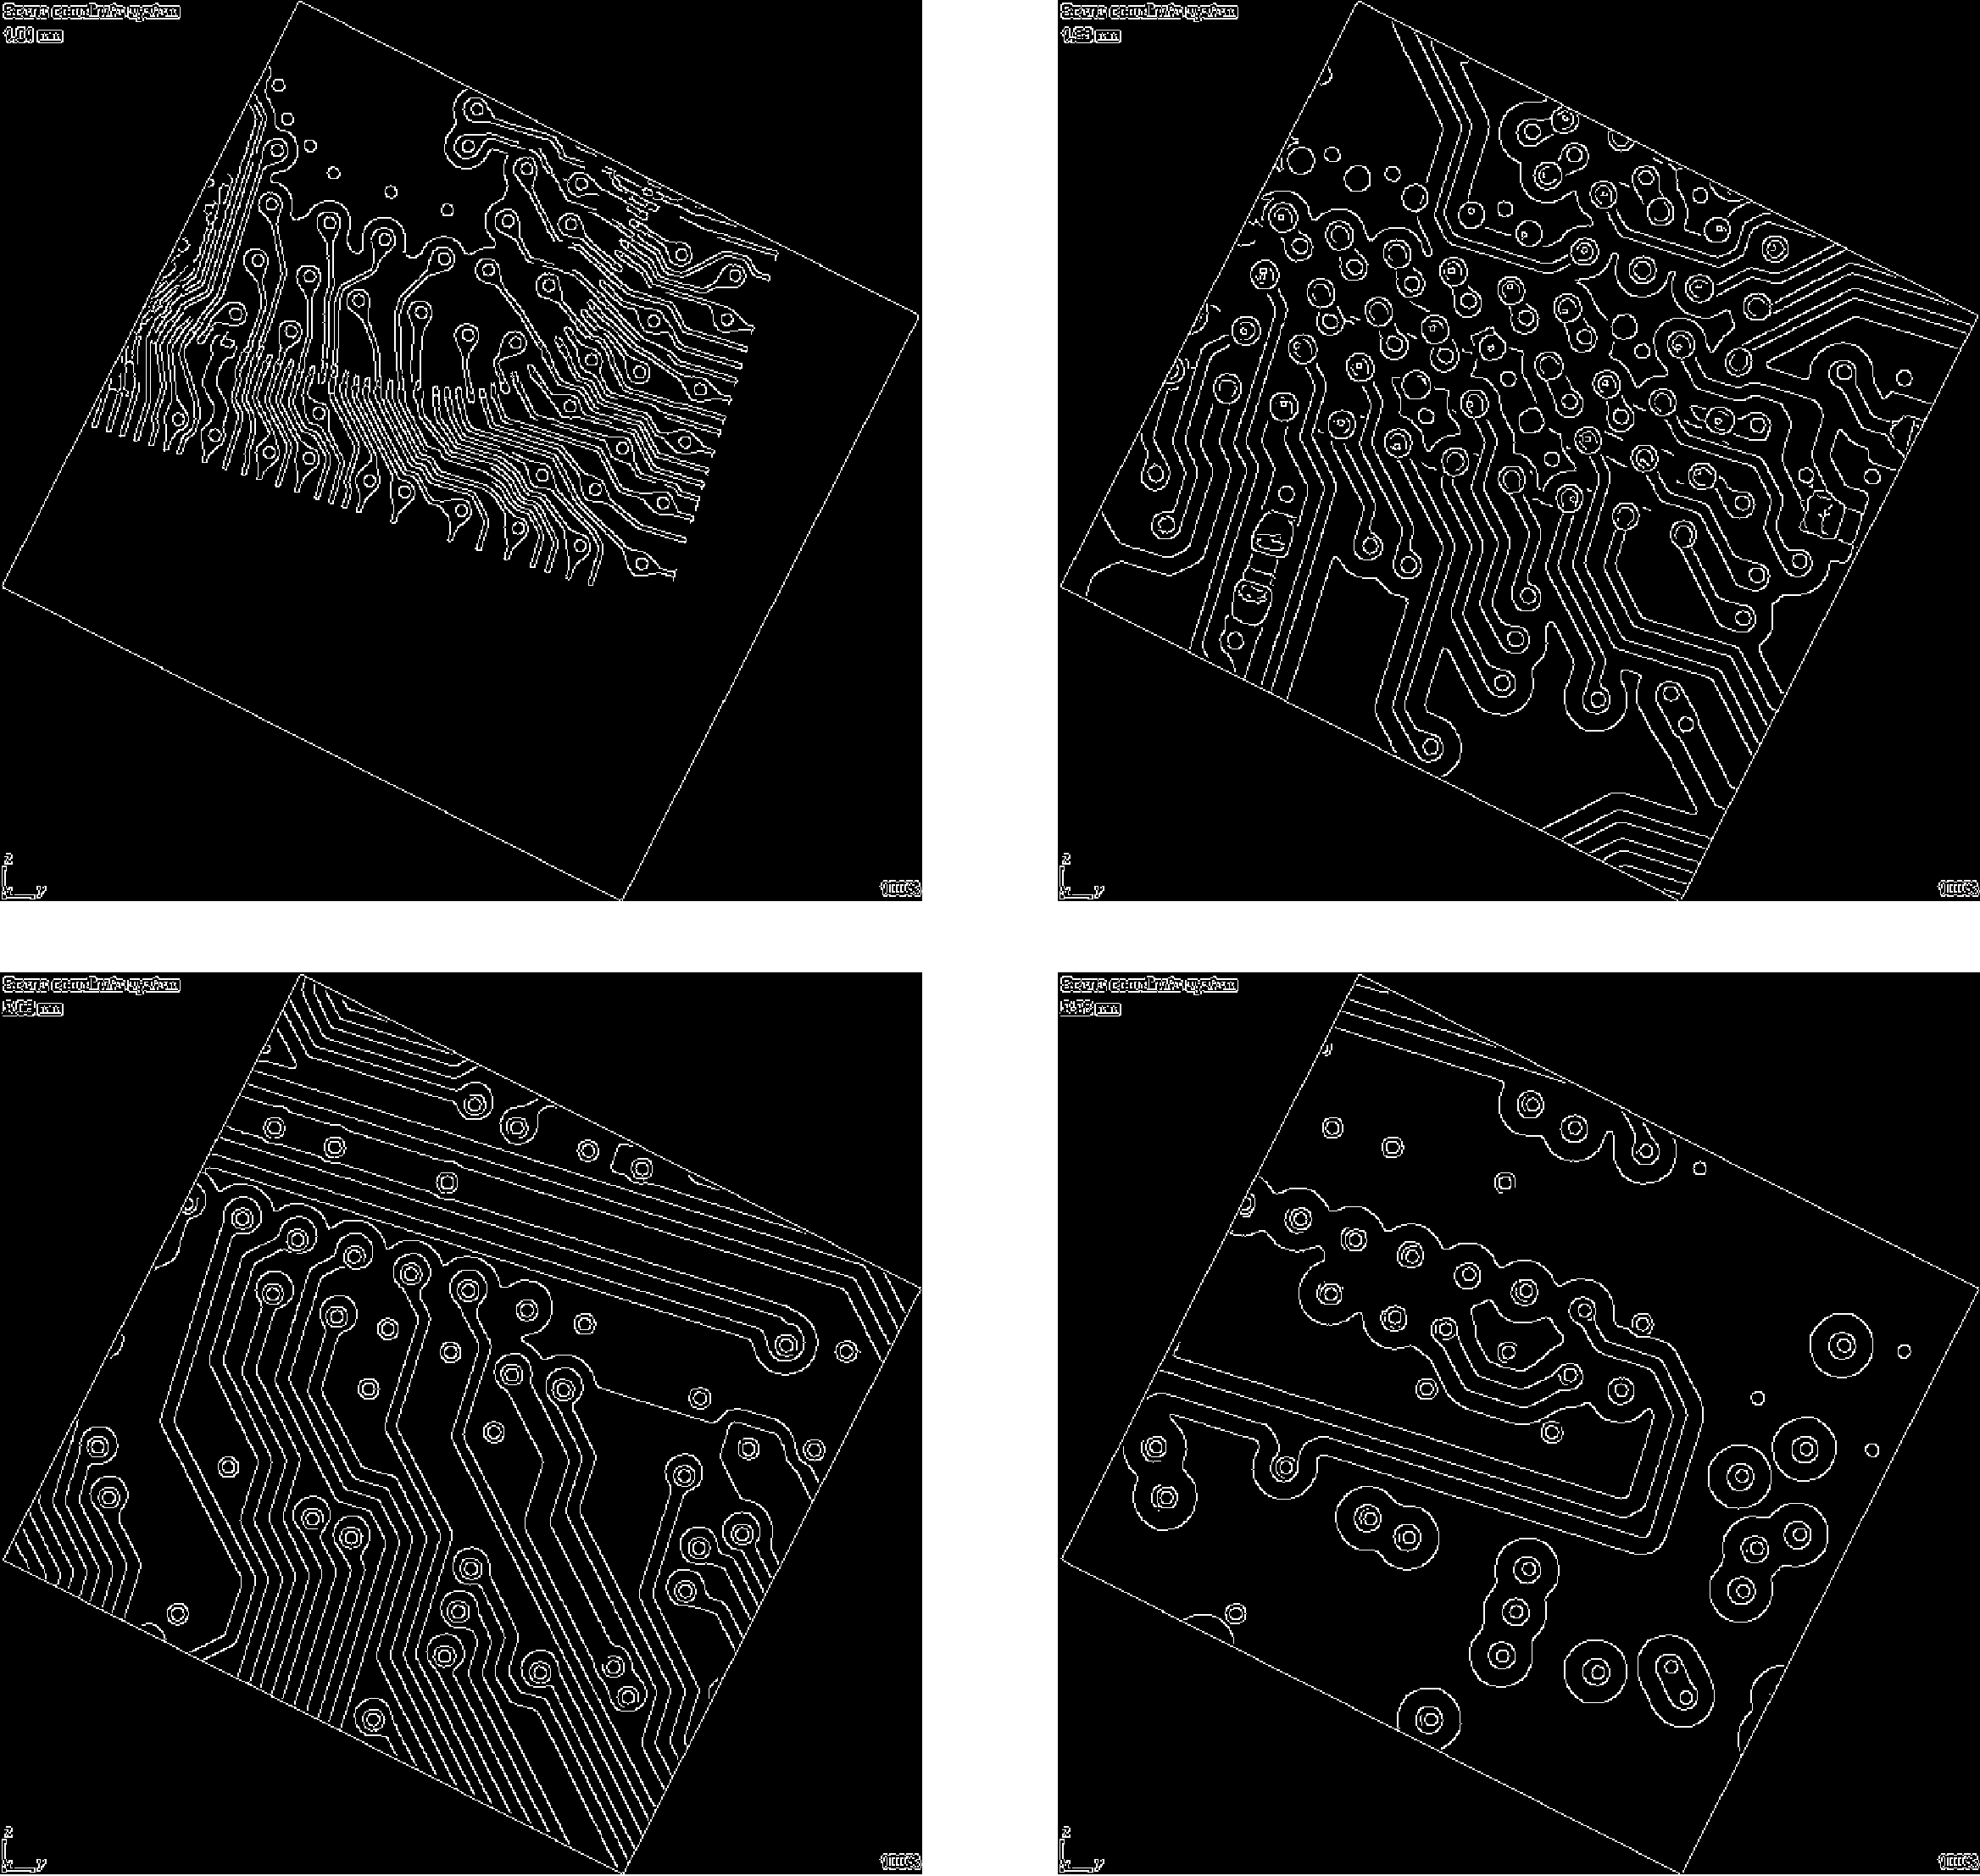
\includegraphics[width=0.9\textwidth]{canny_max_canny_results.pdf}
    \caption{Kantenbilder der Ergebnisse des Canny-Edge-Verfahrens}
    \label{fig:canny_max_bestmatch4}
  \end{center}
\end{figure}

Für die einzelnen Intervalle sind dies die Bilder mit folgenden Indizes:
\begin{enumerate}
	\item{Intervall 1: $Index$ $27$, Differenz zum Best Match: 0}
	\item{Intervall 2: $Index$ $60$, Differenz zum Best Match: 1}
	\item{Intervall 3: $Index$ $83$, Differenz zum Best Match: 0}
	\item{Intervall 4: $Index$ $95$, Differenz zum Best Match: 1}
\end{enumerate}

Dies führt zu einer durchschnittlichen Distanz von \textbf{0,5} vom Best Match.


\section{Hough-Transformation}
Dieses Verfahren ziehlt darauf ab, die Bilder in den Intervallen zu finden, die möglichst gut detektierbare Kantenverläufe, und somit möglichst gut erkennbare Leiterbahnen enthalten. \\
Dafür werden aus den Bildern mit Hilfe der Houghtransformation die Kanten extrahiert und anschließend gezählt. Das Maximum für jedes Intervall ist jenes Bild, welches die meisten zählbaren Kanten enthält.

\subsection{Ergebnis} 

Die Ergebnisse des Verfahrens für die vier Intervalle:
\begin{figure}[H]
  \begin{center}
    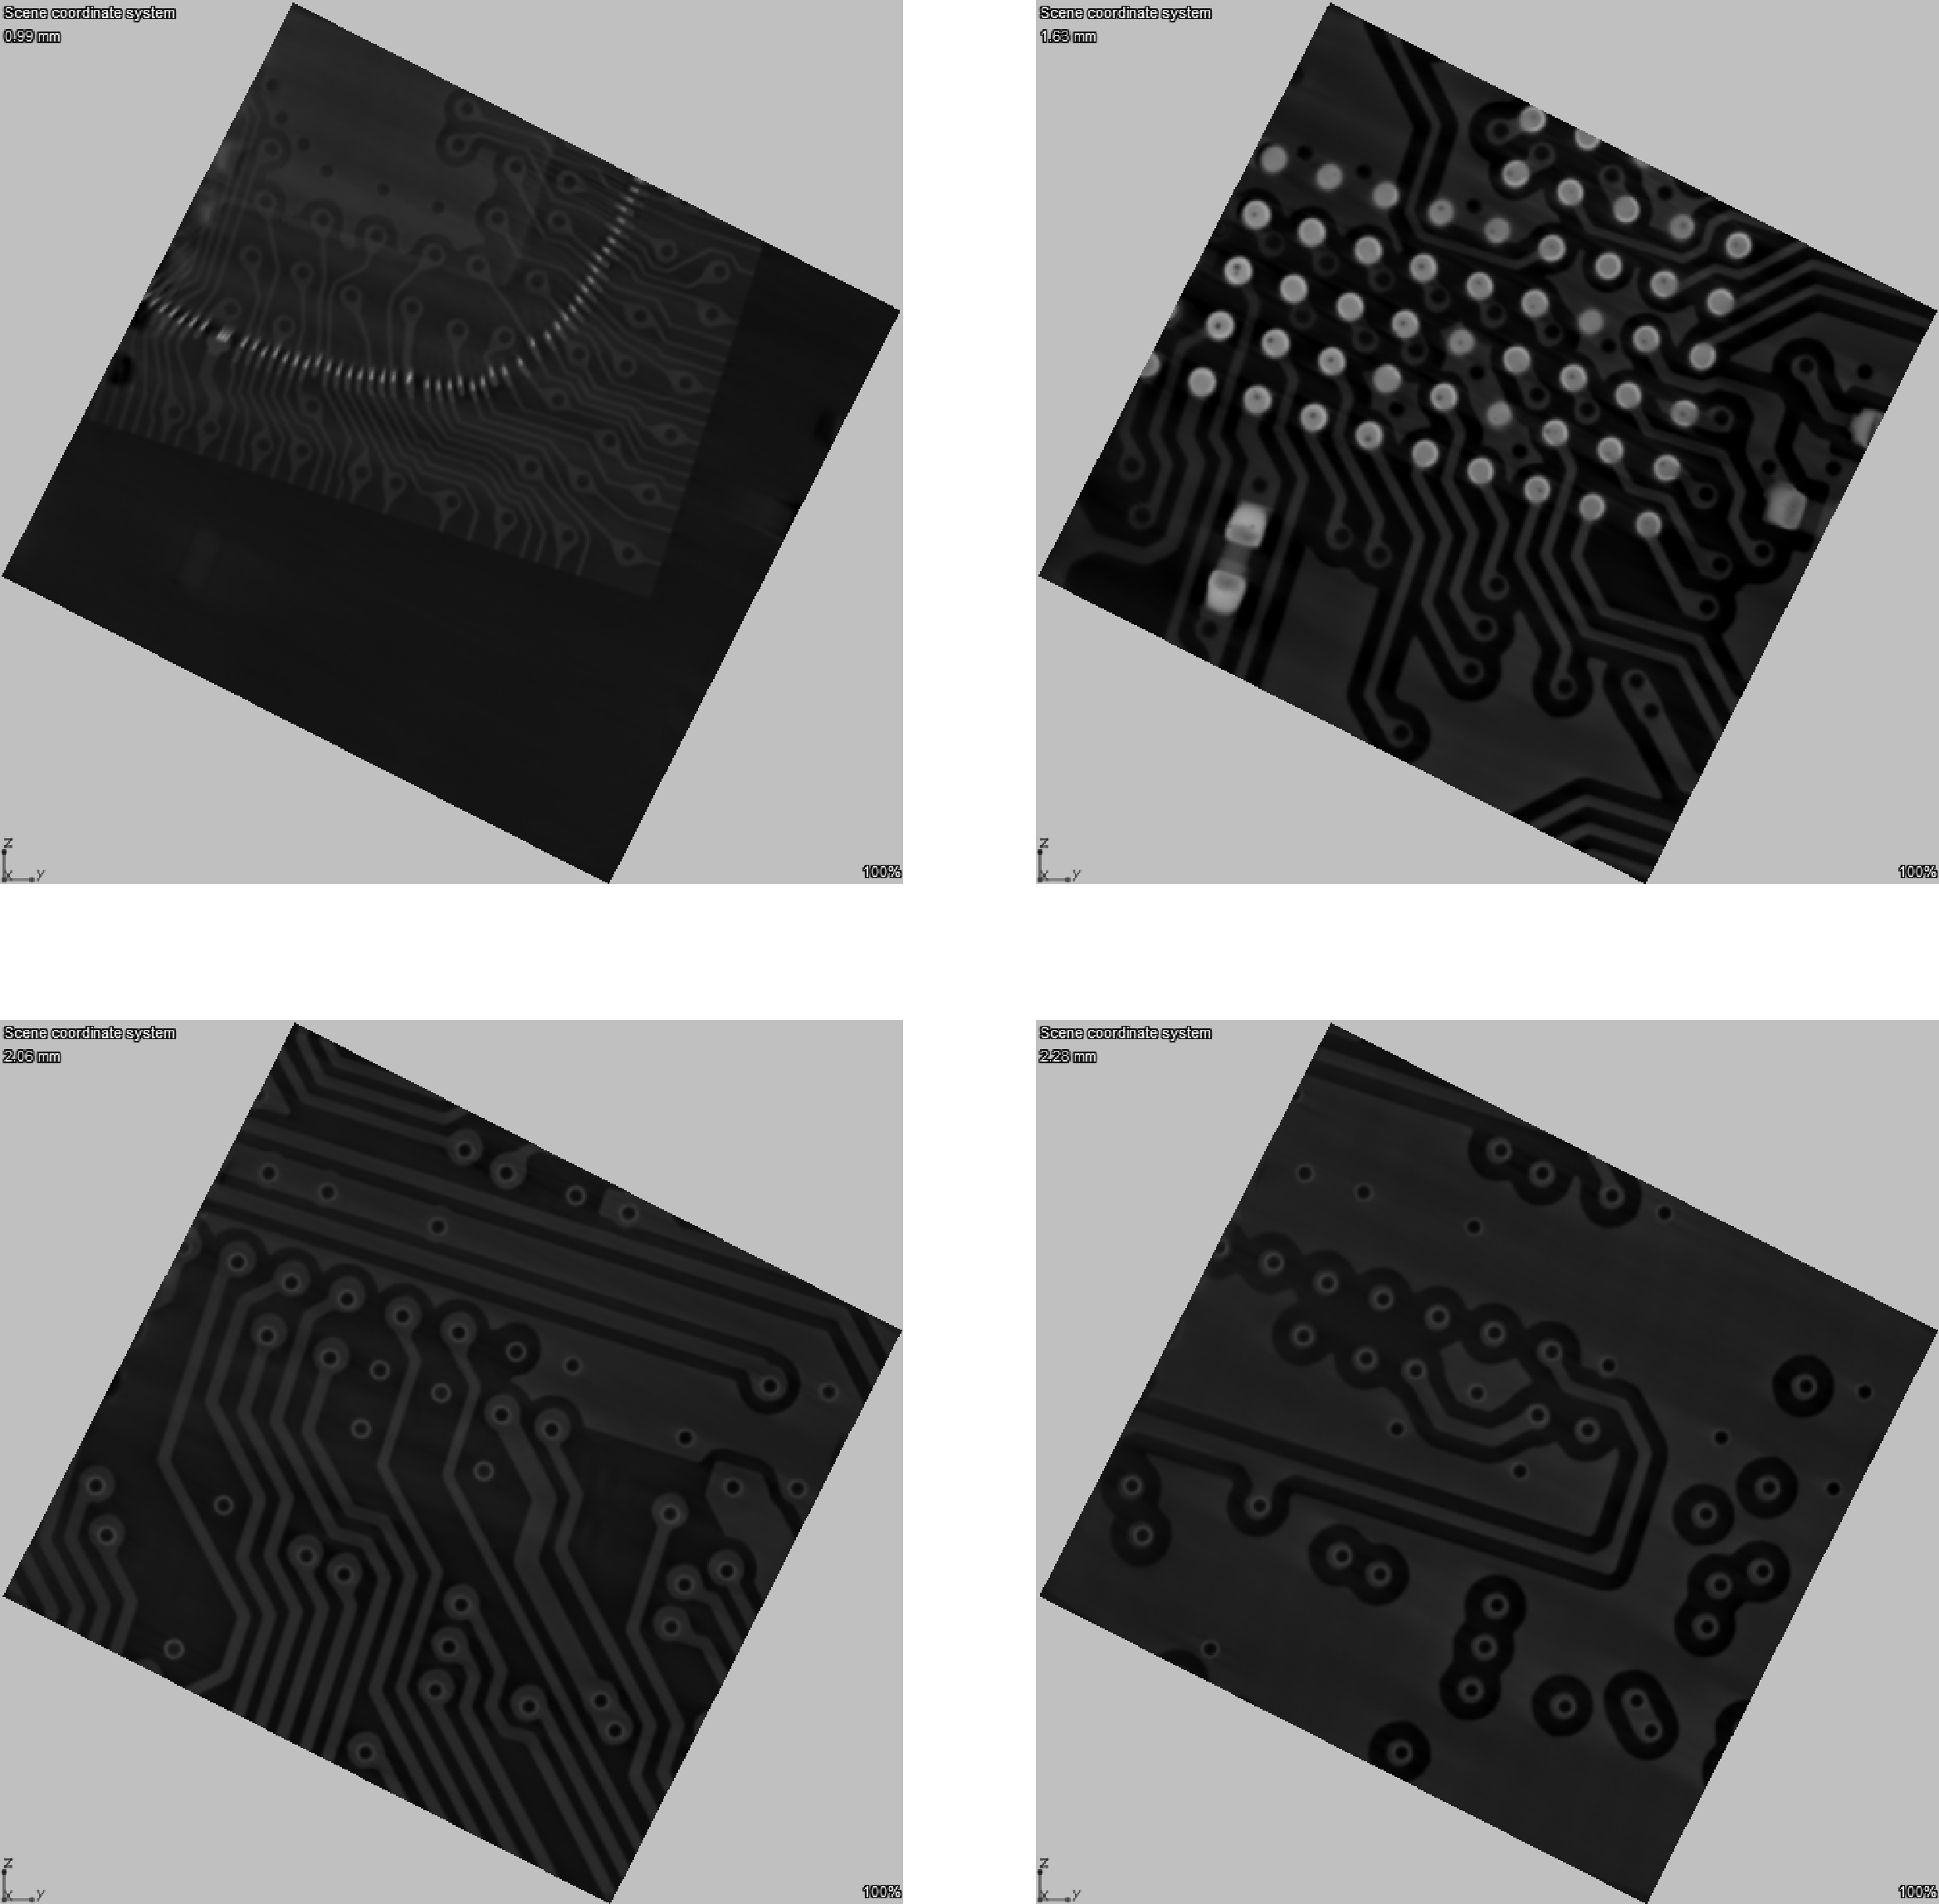
\includegraphics[width=0.9\textwidth]{hough_max.pdf}
    \caption{Ergebnisse des Houghtransformationsverfahrens}
    \label{fig:hough_bestmatch4}
  \end{center}
\end{figure}

Für die einzelnen Intervalle sind dies die Bilder mit folgenden Indizes:
\begin{enumerate}
	\item{Intervall 1: $Index$ $26$, Differenz zum Best Match: 1}
	\item{Intervall 2: $Index$ $60$, Differenz zum Best Match: 1}
	\item{Intervall 3: $Index$ $83$, Differenz zum Best Match: 0}
	\item{Intervall 4: $Index$ $95$, Differenz zum Best Match: 1}
\end{enumerate}

Dies führt zu einer durchschnittlichen Distanz von \textbf{0,75} vom Best Match.

\section{Vergleich}
Es ist deutlich zu erkennen, dass das Binärbildverfahren deutlich schlechtere Ergebnisse (durchschnittliche Distanz: $5,75$) liefert, als das Canny-Edge-Verfahren (durchschnittliche Distanz: $0,5$) und das Houghtransformationsverfahren (durchschnittliche Distanz: $0,75$). Dies liegt vor allem daran, dass Störpixel, bzw. für die weitere Verarbeitung irrelevante Informationen, in Form von nicht defninierten Objekten einen starken Einfluss auf die Menge der weißen Pixel nehmen. Beim Canny-Edge-Verfahren werden primär "`echte"' Objekte, also Objekte, die aus zusammenhängenden Kanten bestehen, extrahiert, während Störpixel bei der Überführung der Bilder in Kantenbilder gefiltert werden. \\
Ein minimal schlechteres Ergebniss liefert das Houghtransformationsverfahren, da dieses Verfahren eine gute Detektierbarkeit der Leiterbahnen berücksichtigt, Bohrpunkte allerdings außer Acht lassen.


